\documentclass[a4paper,14pt]{extarticle}

\usepackage[T2A]{fontenc}
\usepackage[utf8]{inputenc}
\usepackage[english, russian]{babel}

\usepackage[left=30mm, right=10mm, top=20mm, bottom=20mm]{geometry}

\usepackage{tempora}
\usepackage{setspace}
\onehalfspacing

\usepackage{titlesec}
\titleformat{\section}[block]{\bfseries\centering\MakeUppercase}{\thesection.}{1em}{}
\titleformat{\subsection}[block]{\bfseries}{\thesubsection.}{1em}{}
\titleformat{\subsubsection}[block]{\normalsize\bfseries}{\thesubsubsection.}{1em}{}

\renewcommand{\contentsname}{\hfill \textbf{СОДЕРЖАНИЕ} \hfill\null}

\usepackage{indentfirst}
\setlength{\parindent}{1.25cm}

\usepackage{amsmath, amsfonts, amssymb}
\usepackage{graphicx}
\usepackage{caption}
\usepackage{subcaption}
\usepackage{float}
\usepackage{tikz}
\usetikzlibrary{patterns}
\usepackage{cmap}
\usepackage{hyperref}
\usepackage{xcolor}
\usepackage{listings}
\usepackage{paralist}

\definecolor{LightGray}{gray}{0.7}

\lstdefinestyle{code}{
    language=Python,
    basicstyle=\small\ttfamily,
    numbers=left,
    numberstyle=\small\color{LightGray},
    stepnumber=1,
    numbersep=5pt,
    backgroundcolor=\color{white},
    showspaces=false,
    showstringspaces=false,
    showtabs=false,
    tabsize=4,
    captionpos=b,
    breaklines=true,
    breakatwhitespace=false,
    frame=single,
    rulecolor=\color{LightGray},
    linewidth=\linewidth,
    keywordstyle=\color{blue}\bfseries,
    commentstyle=\color{green!40!black},
    stringstyle=\color{violet},
    escapeinside={\%*}{*)},
    xleftmargin=10pt,
    xrightmargin=10pt,
    framexleftmargin=0pt,
    framexrightmargin=0pt
}
\lstset{style=code}

\hypersetup{
    colorlinks=true,
    linkcolor=blue,
    filecolor=magenta,
    urlcolor=cyan,
    pdftitle={ITMO Practice},
    pdfauthor={Rumyantsev Alexey},
    pdfsubject={TCP computer-robot communication},
    pdfkeywords={LaTeX, PDF, robot, tcp},
    pdfpagemode=FullScreen,
}

\graphicspath{{src/images/}}

\begin{document}

\begin{titlepage}
    \begin{center}
        \textbf{Федеральное государственное автономное образовательное учреждение высшего образования}\\
        \textbf{«НАЦИОНАЛЬНЫЙ ИССЛЕДОВАТЕЛЬСКИЙ УНИВЕРСИТЕТ ИТМО»}\medskip\\
        \textbf{Факультет систем управления и робототехники}
        \vfill

        {\large\bfseries Отчет о}\\
        {\large\bfseries научно исследовательской работе}\medskip\\
        {\large\bfseries по теме:}\\
        {\large\bfseries «РАЗРАБОТКА АЛГОРИТМОВ ДЛЯ ВЗАИМОДЕЙСТВИЯ С РОБОТОМ-МАНИПУЛЯТОРОМ С КОМПЬЮТЕРА (С ИСПОЛЬЗОВАНИЕМ TCP)»}
        \vfill

        \begin{flushright}
            Выполнил: студент гр. R3341\\
            А. А. Румянцев\medskip\\

            Проверил: преподаватель\\
            доцент, старший научный сотрудник, инженер В. С. Громов
        \end{flushright}

        \vfill

        Санкт-Петербург\\
        2025 г.
    \end{center}
\end{titlepage}

\setcounter{page}{2}
\tableofcontents
\newpage


\section*{Введение}
\addcontentsline{toc}{section}{Введение}
\setcounter{section}{0}
В настоящее время в промышленной и других сферах все чаще
используются роботы-манипуляторы, управляемые
со специального пульта или автоматически
через загрузку программы на робота.
Более предпочтительным является вариант
управления без человека -- это безопаснее
и выгоднее. Однако роботы используют
достаточно устаревший язык программирования,
например MELFA-BASIC. Написание кода
для подобных роботов может быть неудобным,
а программы получаться громоздкими.
Разработка нового языка программирования
для роботов потребует больших вложений,
что также не выгодно. Управление с пульта,
в свою очередь,
требует от оператора высокой квалификации --
необходимы знания техники безопасности и
принципы работы оборудования. Обучение
специалиста для управления роботом-манипулятором с пульта
является ресурсоемким процессом, требующим
значительных временных и финансовых затрат.


Для повышения безопасности и эффективности
взаимодействия с роботом,
необходимо максимально отдалить человека
от робота, при этом реализовать все основные
функции для работы с ним так, чтобы их можно
было использовать из некой виртуальной централизованной
системы по нажатию кнопок. Реализовать данную идею
можно в виде программного интерфейса -- аналога физического
пульта управления роботом в
виде программы на компьютере.
Такой подход также
позволит упростить обучение специалистов для управления
роботом-манипулятором. Кроме того, программу можно
купить один раз и установить на множество компьютеров,
а разработка и покупка нескольких физических пультов управления
будет ресурсозатратным процессом.
Однако сейчас программных интерфейсов, позволяющих взаимодействовать
с роботом с компьютера сравнительно немного,
а те, что уже есть, постепенно устаревают.
Возникает необходимость написания нового
программного интерфейса для взаимодействия с роботом.
Как и любая другая программа, структурно она делится на две
части -- одна отвечает за внешний вид
и удобство управления (интерфейс),
другая же обеспечивает взаимодействие с роботом
на уровне, не видном пользователю.
В рамках данной работы разрабатывалась
внутрення логика программы для
взаимодействия компьютера с
роботом-манипулятором по протоколу TCP.
Пользовательская часть интерфейса при этом рассматривалась как вспомогательная.


\section{Подготовка к написанию программы}
\subsection{Ознакомление с объектом работы}
Перед выполнением задания был проведен
инструктаж по технике безопасности обращения
с роботом-манипулятором.


Под наблюдением преподавателя
были изучены ручной режим
управления роботом со специального пульта и
автоматический с помощью простейших программ
на языке MELFA-BASIC, загружаемых на робота.


Для написания программ для робота был изучен язык программирования
MELFA-BASIC, некоторые его основные команды и описание представлены
далее:
\begin{compactitem}
    \item \textbf{SERVO ON} -- включение двигателей,
    \item \textbf{SERVO OFF} -- выключение двигателей,
    \item \textbf{END} -- завершение программы, обязательно размещается в конце файла,
    \item \textbf{JOVRD 100} -- скорость движения в процентах от максимальной,
    \item \textbf{SPD 100} -- скорость движения при интерполяционных командах,
    \item \textbf{MOV P1} -- движение в заданную точку P1,
    \item \textbf{WHILE, FOR} -- циклы с условиями,
    \item \textbf{OPEN "COM3:" AS \#1} -- открытие TCP/IP порта 10003 для подключения интерфейса \#1,
    \item \textbf{CLOSE \#1} -- закрытие TCP/IP порта 10003 для подключения интерфейса \#1,
    \item \textbf{DEF INTE DCOMM} -- объявление переменной DCOMM целочисленного типа.
\end{compactitem}


\subsection{Выбор подходящего языка программирования}
Существует достаточно много различных языков программирования,
подходящих под реализацию задачи взаимодействия с роботом с
компьютера. В рамках данной работы был выбран язык
программирования Python, так как он достаточно часто
используется в сфере робототехники, имеет достаточно простой
и легкочитаемый синтаксис,
имеет большое количество готовых библиотек и является кроссплатформенным
(программу можно запустить на разных операционных системах).


В ходе выполнения работы использовались следующие библиотеки:
\begin{compactitem}
    \item \textbf{socket} -- для работы с сетевыми соединениями,
    \item \textbf{typing} -- средства для статической типизации переменных и функций,
    \item \textbf{re} -- модуль для работы с регулярными выражениями,
    \item \textbf{yaml} -- для чтения и записи файлов в формате YAML,
    \item \textbf{enum} -- позволяет создавать перечисления с именованными значениями.
\end{compactitem}


Библиотека socket понадобилась для установки TCP-соединения между компьютером и роботом
и передачи/получения пакетов.


Для общего улучшения и упрощения кода использовалась
библиотека typing.


Модуль re понадобился для обработки ответов с робота.


Библиотека
yaml позволила реализовать чтение и сохранение введенных настроек IP и порта, чтобы
пользователю не пришлось каждый раз вводить эти данные заново при запуске программы.


Для перечисления команд, статусов сетевого взаимодействия с роботом,
декартовых и сочлененных координат понадобилась библиотека enum.


\section{Реализация программы для взаимодействия компьютера с роботом-манипулятором}
\subsection{Определение формата сообщения}
Для начала необходимо определиться
с форматом передаваемого с компьютера
на робот-манипулятор сообщения и обратно.


Сообщение должно быть простое, соответствующее
шаблону которое понимает робот.


Сначала будет отправляться номер команды, после чего
шесть координат и пара чисел для решения
обратной задачи кинематики, если хотим
передвижение по декартовым координатам.
Если движение сочлененное, то достаточно
передать шесть углов вращения.


Было решено, что робот будет отправлять компьютеру
12 координат и пару для решения обратной задачи кинематики
как одно сообщение (изменение декартовых координат влияет на сочлененные и наоборот).


В ходе выполнения работы экспериментальным путем было выяснено, что
робот отправляет свои декартовы и сочлененные координаты
в следующем формате:
$$
['(J_1,J_2,J_3,J_4,J_5,J_6)(X,Y,Z,A,B,C)(K_1,K_2)'],
$$
то есть как список, содержащий одну строку.


Это означает, что роботу нужно отправлять
координаты в виде строк шаблона:
\begin{compactitem}
    \item $(J_1,J_2,J_3,J_4,J_5,J_6)$ -- если движение сочлененное,
    \item $(X,Y,Z,A,B,C)(K_1,K_2)$ -- если движение в декартовых координатах,
\end{compactitem}
при этом все значения с плавающей точкой, кроме $K_i$ -- они целочисленные.


\subsection{Определение основных команд}
Проще всего отправлять роботу не строковые команды вида 'EXIT',
а численные в виде строк. Например, команда '0' -- завершение работы
робота.


Создадим для удобства перечисление enum, где каждой
команде с названием будет присвоено собственное число.
\begin{lstlisting}[label=robocmd, caption={Определение перечисления с командами для робота.}]
class RobotCommand(Enum):
    EXIT = 0
    GET_POSITION = 1
    MOVE_LINEAR = 2
    MOVE_JOINTS = 3
\end{lstlisting}


Краткое описание команд:
\begin{compactitem}
    \item \textbf{'0'} -- завершение работы робота. На клиентской стороне отключение связи,
    \item \textbf{'1'} -- робот вышлет 12 своих координат и кинематическую пару,
    \item \textbf{'2', '3'} -- движение робота по декартовым координатам или сочлененное соответственно.
    После робот снова высылает свою позицию.
\end{compactitem}


В программе для робота будем проверять пришедшее сообщение
на совпадение с одним из этих чисел. Далее будет
выполняться соответствующий алгоритм.


Например, при получении
'2' робот будет двигаться по декартовым координатам в соответствии
с присланной после команды в заданном шаблоне следующей позицией робота, после чего
вышлет обратно 12 своих координат и пару чисел для решения
обратной задачи кинематики.


\subsection{Клиентская программа для общения с роботом}
Напишем клиентский скрипт, который будет основой сетевеого взаимодействия
компьютера с роботом.


Для начала определим статусы сетевого взаимодействия как перечисление.
Они помогут при отладке ошибок.
\begin{lstlisting}[label=lst:constat, caption={Определение перечисления статусов соединения компьютера с роботом.}]
class ConnectionStatus(Enum):
    SUCCESS = auto()
    NOT_CONNECTED = auto()
    CONNECTION_ERROR = auto()
    SEND_ERROR = auto()
    RECEIVE_ERROR = auto()
    NONE = auto()
\end{lstlisting}


Нумерация статусов автоматически с 1 и по порядку.
Смысл статусов полностью соответствует их названиям.


Теперь реализуем основные функции для взаимодействия компьютера с роботом.
Полностью скрипт представлен в приложении А на листинге \ref{lst:client}.


Краткое описание функций скрипта:
\begin{compactitem}
    \item \textbf{\_\_init\_\_(self)} -- при создании объекта класса вызывается
    данная функция. Она присвоит объекту поля: sock -- сетевой сокет с параметрами
    AF\_INET (семейство адресов IPv4), SOCK\_STREAM (протокол TCP);
    булевое connected -- значение истина или ложь в зависимости от
    того, подключен ли сокет к указанному IP и порту;
    \item \textbf{connect(self, ip: str, port: int) -> ConnectionStatus} --
    подключение сокета к указанному IP адресу и порту. Возвращает
    статус соединения. Также присваивает значение "истина"\,
    переменной connected, если подключение удалось;
    \item \textbf{disconnect(self) -> ConnectionStatus} -- закрывает
    соединение, если оно есть. Возвращает статус соединения.
    \item \textbf{send(self, data: str) -> ConnectionStatus} --
    кодирует переданную строку сообщение data и отправляет по
    протоколу TCP. Возвращает статус соединения;
    \item \textbf{receive(self, out\_data: list, buffer\_size: int = 1024) -> ConnectionStatus}
    -- принимает данные по протоколу TCP. Записывает в декодированном виде
    полученную информацию в список out\_data. Возвращает статус соединения.
\end{compactitem}


\subsection{Программа на роботе для общения с клиентом}
На языке MELFA-BASIC напишем простую программу для теста
связи между компьютером и роботом:
\lstdefinelanguage{BASIC}{
  morekeywords={PRINT,MOV,CLOSE,SERVO,INPUT,IF,ENDIF,WEND,THEN,ELSE,FOR,TO,NEXT,GOTO,END,REM,WHILE,JOVRD,SPD,DEF,INTE,OPEN},
  sensitive=false,
  morecomment=[l]{REM},
  morestring=[b]",
}
\begin{lstlisting}[language=Basic, label=lst:mbtest, caption={Простая программа на роботе для проверки связи с клиентом.}]
JOVRD 100
SPD 100
DEF INTE DCOMM
DCOMM = 1
PHELP = P_CURR
SERVO ON
OPEN "COM3:" as #1

WHILE DCOMM > 0
    INPUT #1, DCOMM
    IF DCOMM = 2 THEN
        INPUT #1, PHELP
        PRINT #1, PHELP
    ENDIF
WEND

CLOSE #1
SERVO OFF
END
\end{lstlisting}


Краткое описание программы: в переменную DCOMM ожидается поступление
номера команды от компьютера. Когда команда '2' пришла, робот
записывает приходящие следующим же сообщением от компьютера
декартовы координаты и кинематическую пару, после чего
высылает обратно то же самое, что и получил.


Если прислали команду '0', то робот выйдет из цикла и завершит работу.


Таким образом проверяется, что робот корректно обрабатывает
полученные координаты, компьютер верно получает те же координаты обратно.
После чего робот успешно завершает работу.


\subsection{Проверка связи между компьютером и роботом}
Сообщение роботу нужно отправить в определенном формате.
Также ответ от робота нужно обработать. Для этого
напишем скрипт, который будем использовать каждый раз перед
отправкой и получением координат. Полностью скрипт
представлен на листинге \ref{lst:cmdman} в приложении Б.


Краткое описание скрипта:
\begin{compactitem}
    \item \textbf{build\_position\_request(pos: List[float]) -> str} --
    на вход получает координаты как список чисел с плавающей точкой.
    Преобразует список в строку в соответствии с шаблоном $\left( v_1,v_2,v_3,v_4,v_5,v_6 \right)$.
    Возвращает результат преобразования;
    \item \textbf{parse\_position\_response(response: list)} --
    получает ответ от робота в виде списка из строки с 12 координатами
    и кинематической пары и с помощью регулярного выражения
    делит строку внутри списка на три отдельных списка из сочлененных
    и декартовых координат и кинематической пары. Возвращает кортеж
    из трех соответствующих списков.
\end{compactitem}


Также нам нужен скрипт для записи и хранения IP и порта робота.
Создадим yaml файл, в котором запишем:
\begin{lstlisting}[label=yaml, caption={Файл, где хранятся данные для подключения к роботу-манипулятору.}]
connection:
  ip: "192.168.0.4"
  port: 10003
\end{lstlisting}


Напишем скрипт, в котором во время работы программы будут сохранены
эти данные. Полностью скрипт представлен в приложении В на листинге \ref{lst:cfg}.


Краткое описание скрипта:
\begin{compactitem}
    \item \textbf{load(cls, path: str = "config.yaml")} -- загружает
    IP адрес и порт из файла по указанном пути. Сохраняет в свои поля ip, port.
    По умолчанию файл находится в том же каталоге, где и скрипт;
    \item \textbf{save(cls, path: str = "config.yaml")} -- сохраняет
    конфигурацию IP и порта в файл по указанному пути;
    \item \textbf{set\_config(cls, ip: str, port: int)} -- меняет
    конфигурацию IP и порта во время работы программы. Может пригодиться,
    если необходимо будет отключиться от одного робота и подключиться к другому,
    не закрывая программу.
\end{compactitem}


Напишем простую программу для компьютера для проверки соединения
с роботом:
\begin{lstlisting}[label=lst:testpy, caption={Простая программа на клиенте для проверки соединения с роботом.}]
import socket
from config_manager import Config
from command_manager import CommandMessageManager

if __name__ == "__main__":
    Config.load()

    pos = [100.0, -100.0, 100.0, 100.0, 100.0, 100.0]
    test = CommandMessageManager.build_position_request(pos)
    test += "(7,0)"
    s = socket.socket(socket.AF_INET, socket.SOCK_STREAM)
    s.connect((Config.ip, Config.port))
    s.sendall("2".encode('utf-8'))
    s.sendall(test.encode('utf-8'))
    ans = s.recv(1024).decode('utf-8')
    print(ans)
    s.sendall("0".encode('utf-8'))
    s.close()
\end{lstlisting}


Краткое описание программы: загружается конфигурация IP и порта
из файла. Задается некоторый набор из шести координат, из которого создается строка
на отправку. Так как отправляются декартовы координаты, необходимо
еще к строке на отправку добавить в строковом виде в таком же
формате кинематическую пару. После чего создается сокет
с полученными из файла IP адресом и портом. Отправляется закодированная команда '2',
за которой следуют закодированные обработанные декартовы координаты.
После чего принимается, декодируется и выводится в консоль ответ от робота.
В конце высылается закодированная команда '0' для завершения работы робота.
На клиенте же закрывается сокет.


В присутствии преподавателя на робота была загружена программа,
представленная на листинге \ref{lst:mbtest}. На компьютере
была запущена программа, представленная на листинге \ref{lst:testpy}.


Было выслано с компьютера:
$$
\left( 100.0, -100.0, 100.0, 100.0, 100.0, 100.0\right)\left( 7,0 \right)
$$


Было получено от робота:
$$
\left( +100.0, -100.0, +100.0, +100.0, +100.0, +100.0\right)\left( 7,0 \right)
$$


Робот и компьютер взаимодействуют корректно -- на компьютер пришло то же,
что было с него выслано. Появились дополнительные плюсы, которые при
обработке ответа от робота пропадут, то есть они незначащие. Ответ
робота был выведен в консоль в сыром виде.


\subsection{Клиентская программа для управления роботом}
Доработаем нашу программу скриптами с функциями,
позволяющими полноценно взаимодействовать
с роботом с компьютера.


Для начала введем перечисления для декартовых и сочлененных координат.


После обработки ответа робота мы получаем, например, список из шести
декартовых координат. Чтобы подвинуться по какой-то из координат,
необходимо добавить шаг к этой координате. Координаты в списке
располагаются по порядку. Значит, при обращении к нулевому элементу
получим первую координату $X$, при обращении к пятому получим шестую координату $C$.
Аналогично с сочлененными координатами.
\begin{lstlisting}[label=lst:coords, caption={Определение перечислений, где каждой координате соответствует свой индекс в списке.}]
class CartesianAxis(Enum):
    X = 0
    Y = 1
    Z = 2
    A = 3
    B = 4
    C = 5

class JointAxis(Enum):
    J1 = 0
    J2 = 1
    J3 = 2
    J4 = 3
    J5 = 4
    J6 = 5
\end{lstlisting}


Также зададим тип координатам. Есть декартовы линейные, декартовы вращательные и сочлененные координаты.
\begin{compactitem}
    \item Линейные декартовы координаты $X,Y,Z$ -- mode: cartesian\_linear,
    \item Вращательные декартовы координаты $A,B,C$ -- mode: cartesian\_rotation,
    \item Сочлененные координаты $J_1...J_6$ -- mode: joint\_rotation.
\end{compactitem}


Для определения команды из перечисления по ее типу напишем такой словарь:
\begin{lstlisting}[label=lst:md2cmd, caption={Словарь для приведения типа координаты к команде из перечисления.}]
MODE_TO_COMMAND = {
    "cartesian_linear": RobotCommand.MOVE_LINEAR,
    "cartesian_rotation": RobotCommand.MOVE_LINEAR,
    "joint_rotation": RobotCommand.MOVE_JOINTS,
} 
\end{lstlisting}


Нам необходимо в программе на компьютере
где-то хранить координаты робота и кинематическую пару.
Создадим виртуального робота на клиенте. Скрипт
расположен в приложении Г на листинге \ref{lst:virtualrobot}.


Краткое описание функций скрипта:
\begin{compactitem}
    \item \textbf{\_\_init\_\_(self, cartesian: ..., joint: ..., kin\_sol: ...)} --
    при создании объекта класса в качестве его полей можно указать декартовы и сочлененные координаты и кинематическую пару.
    Иначе они будут заданы нулевыми;
    \item \textbf{update\_cartesian(self, new\_values: ..., kinematic\_sol: ...)} --
    обновляет декартовы координаты и кинематическую пару виртуального робота;
    \item \textbf{update\_joint(self, new\_values: ...)} -- обновляет сочлененные
    координаты виртуального робота;
    \item \textbf{calculate\_next\_move(self, mode: ..., axis\_index: int, step: float) -> ...} --
    проверяет тип координаты и считает соответствующие следующие координаты робота. Функция принимает тип координаты, ее индекс
    в списке координат и шаг, на который нужно сдвинуть робота по этой координате (миллиметры для линейных координат,
    градусы для вращательных). Возвращает список соответствующих координат, где одно из значений смещено на некоторый шаг.
\end{compactitem}


Так как обратная задача кинематики на клиенте не решается, то кинематическая пара
нужна только для того, чтобы выслать ее обратно вместе с декартовыми координатами роботу.


В интерфейсе подразумевается наличие кнопок каждой координаты в двух типах: со знаком минус и со знаком плюс.
Для упрощения логики программы введем кортеж, который будем называть move\_info. В нем будут содержаться
тип координаты, ее порядковый номер в списке и направление, задаваемое знаком плюс или минус. Примеры
кортежей приведены далее.
\begin{compactitem}
    \item \textbf{("cartesian\_linear"\,, CartesianAxis.X.value, '+')} -- декартова линейная координата $X$, порядковый номер
    определяется перечислением декартовых координат (в этом случае будет 0) и положительное направление;
    \item \textbf{("cartesian\_rotation"\,, CartesianAxis.A.value, '-')} -- декартова вращательная координата $A$, порядковый
    номер в списке определяется аналогично (в данном случае 4) и отрицательное направление;
    \item \textbf{("joint\_rotation"\,, JointAxis.J1.value, '+')} -- сочлененная вращательная координата $J_1$,
    порядковый номер 0 и положительное направление.
\end{compactitem}


Теперь для всего, что мы уже написали на клиенте, нужна простая надслойка -- скрипт,
функции которого будут объединять несколько действий, необходимых для полноценного взаимодействия
с роботом. Эту надслойку можно будет использовать, например, в обработчиках нажатия кнопок в графическом интерфейсе.
Скрипт представлен в приложении Д на листинге \ref{lst:backctrl}.


Краткое описание функций данного скрипта:
\begin{compactitem}
    \item \textbf{\_\_init\_\_(self)} -- создает объект класса и
    присваивает поля: robot -- виртуальный робот, client -- клиентская
    обертка над сокетом и last\_...\_status -- статус сетевого взаимодействия для каждой
    последней операции компьютера с роботом (присоединение, отправка, получение и отключение;
    может пригодиться для удобной отладки сетевых проблем). Далее во всех функциях присваивание
    сетевых статусов аналогичное;
    \item \textbf{connect(self, ip: str, port: int)} -- обертка подключения над клиентской
    оберткой подключения над сокетом. Возвращает булевую переменную connected объекта класса Client.
    Дополнительная обертка позволяет при необходимости добавить некоторую
    логику до прямого соединения с роботом;
    \item \textbf{disconnect(self)} -- обертка отключения над клиентской
    оберткой отключения над сокетом. Возвращает отрицание булевой переменной connected объекта класса Client.
    В функцию до прямого отключения от робота дополнительно добавлена логика оповещения робота,
    что клиент отключается -- высылается команда '0' для завершения работы робота;
    \item \textbf{is\_connected(self)} -- возвращает булевую переменную connected объекта класса Client.
    Непрямая проверка соединения. Есть возможность добавить дополнительную логику;
    \item \textbf{get\_pos(self)} -- высылает команду '1' роботу, чтобы получить
    его текущие координаты и кинематическую пару. Возвращает ответ робота без обработки.
    Подразумевается, что обработка будет сделана извне этой функции, ее методы могут быть любыми
    в соответствии с нуждами;
    \item \textbf{move\_axis(self, move\_info: ..., step: float)} -- принимает кортеж
    из трех элементов, описанных ранее, и шаг. По направлению определяет знак шага.
    Вызывает функцию calculate\_next\_move виртуального робота, куда передает тип координаты,
    ее порядковый номер и шаг (подразумевается, что в виртуальном роботе уже сохранены координаты
    настоящего). Далее отправляет на робот номер команды в соответствии
    с конвертацией из словаря MODE\_TO\_COMMAND. С помощью build\_position\_request
    создает сообщение роботу с новыми координатами, полученными от виртуального робота.
    Если тип координат декартовый, то добавляет в конец сообщения кинематическую пару
    в соответствии с форматом сообщения. После этого отправляет номер команды и координаты.
    Получает ответ от робота и возвращает его без обработки.
\end{compactitem}


Алгоритмы на клиенте готовы. Осталось написать алгоритм на роботе
и добавить интерфейс с кнопками.


\subsection{Программа управления робота при взаимодействии с клиентом}
Напишем программу для робота на языке MELFA BASIC для реализации
выполнения роботом команд, присылаемыех с клиента. Полностью программа
представлена в приложении Е на листинге \ref{lst:finalmelfa}.


Краткое описание программы: робот ждет номер команды в переменную DCOMM.
Есть вспомогательные переменные, куда будут записываться приходящие с клиента
координаты -- PHELP для декартовых, JHELP для сочлененных. Пока на робота не отправили
команду '0', он в цикле ждет следующую команду. При получении команды '1', робот
вышлет обратно свои текущие 12 координат и кинематическую пару. Если придет команда '2',
то робот примет декартовы координаты и кинематическую пару сразу после команды, с помощью MOV переместится
в новые декартовы координаты, далее отправит ответ о своих текущих координатах (они должны
соответствовать тем, что были отправлены). Аналогично при получении команды '3', однако
координаты сочлененные и не нужна кинематическая пара. Если приходит команда '0', то
цикл завершается, робот выключается, предварительно закрыв соединение.


\section{Добавление пользовательского интерфейса}
Данная практическая работа является частью общего проекта
на тему "Разработка графического интерфейса для взаимодействия с\\ роботом-манипулятором".
Этот проект делится на две подтемы -- тема данной работы и "Разработка графического интерфейса программы".
Вторая подтема была выполнена студентом, с которым выполнялся общий проект.
Следовательно, в данной практической работе пользовательская часть интерфейса
не будет подробно рассматриваться, так как в данной теме она является вспомогательной.
Разработанные алгоритмы взаимодействия с роботом возможно использовать в различных
графических интерфейсах.


\subsection{Описание интерфейса}
Краткое описание интерфейса: в интерфейсе
есть кнопки на каждую координату в двух видах -- с плюсом и с минусом.
Шаг задается ползунками -- в миллиметрах для линейных координат, в градусах для вращательных координат.
Есть возможность задавать и менять IP адрес и порт в окне программы. Есть кнопка подключения,
которая после успешного подключения меняется на кнопку отключения. Пока подключение к роботу
не осуществлено, интерфейс остается недоступным.


\subsection{Взаимодействие интерфейса и основной логики программы}
Рассмотрим взаимодействие интерфейса и основной логики программы.


Каждой кнопке в окне программы соответствует свой move\_info.
Структурно это словарь, который можно назвать картой кнопок окна программы.
Реализация представлена на листинге \ref{mvinf} в приложении Ж.


При полном нажатии кнопки connect, вызывается функция обработки
нажатия данной кнопки handle\_connection(self). Ее реализация
представлена на листинге \ref{lst:hancon} в приложении З.


Краткое описание функции handle\_connection(self):
проверяет функцией is\_connected, есть ли подключение
компьютера к роботу. Если подключения нет (например, первый запуск программы),
то берется сохраненная конфигурация IP и порта, вызывается функция connect
у надслойки. Если подключение не удалось, то интерфейс останется заблокированным.
Чтобы снова попытаться подключиться, необходимо будет нажать кнопку connect еще раз.
Если подключение удалось, то на робот сразу высылается запрос на получение
координат через функцию надслойки get\_pos. Далее ответ обрабатывается
функцией parse\_position\_response. После обработки полученные координаты
и кинематическая пара присваиваются виртуальному роботу, также вызывается
функция обновления отображаемых в интерфейсе координат робота. Эта функция
берет координаты из виртуального робота и выводит их в окно программы.
В конце интерфейс разблокируется, кнопка connect меняется на disconnect.
Если подключение уже есть и кнопка нажата еще раз, то произойдет отключение
клиента от робота через надслойку disconnect, то есть на робот будет
отправлена команда '0' и он выключится.



При нажатии кнопок изменения координат вызывается обработчик\\
handle\_axis\_button(self). Реализация данной функции представлена
на листинге \ref{lst:hab} в приложении И.


Краткое описание функции handle\_axis\_button(self):
берет из карты кнопок с move\_info кортеж move\_info по имени нажатой кнопки.
Проверяет, какой тип координаты находится в этом кортеже. Если тип декартовый линейный,
то берет шаг с ползунка с миллиметровой шкалой. Если тип декартовый вращательный,
то берет шаг с ползунка для декартовых вращательных координат с градусной шкалой.
Если тип сочлененный, то аналогично декартовым вращательным координатам, но
ползунок для сочлененных координат. Далее вызывает функцию move\_axis, куда передает
move\_info и шаг,
обрабатывает ответ функцией parse\_position\_response, записывает
в виртаульного робота пришедшие от настоящего координаты и кинематическую пару.
Далее вызывает функцию обновления координат в интерфейсе.


\section{Тестирование работы программы}
\subsection{Проверка работы программы}
Для тестирования напишем основной файл, где будет вызываться интерфейс:
\begin{lstlisting}[label=lst:main, caption={Точка входа программы.}]
import sys
from PySide6.QtWidgets import QApplication
from config_manager import Config

import main_window as mw

if __name__ == "__main__":
    Config.load()

    app = QApplication(sys.argv)

    window = mw.MainWindow()
    window.show()

    sys.exit(app.exec())
\end{lstlisting}


Сначала загружается конфиг IP и порта, после создается окно программы,
к кнопкам которого привязана логика взаимодействия компьютера с роботом по TCP.


Все опыты проводились в присутствии преподавателя.
На робот загружена программа, представленная на листинге \ref{lst:finalmelfa}.
Подключение робота к ноутбуку осуществлялось через Ethernet кабель.


Окно клиентской программы до подключения к роботу имеет вид, представленный на рис. \ref{fig:nonactive}.
После успешного подключения клиентской программы к роботу, окно
программы принимает вид, представленный на рис. \ref{fig:active_cartesian}, \ref{fig:active_joint}.
\begin{figure}[H]
    \centering
    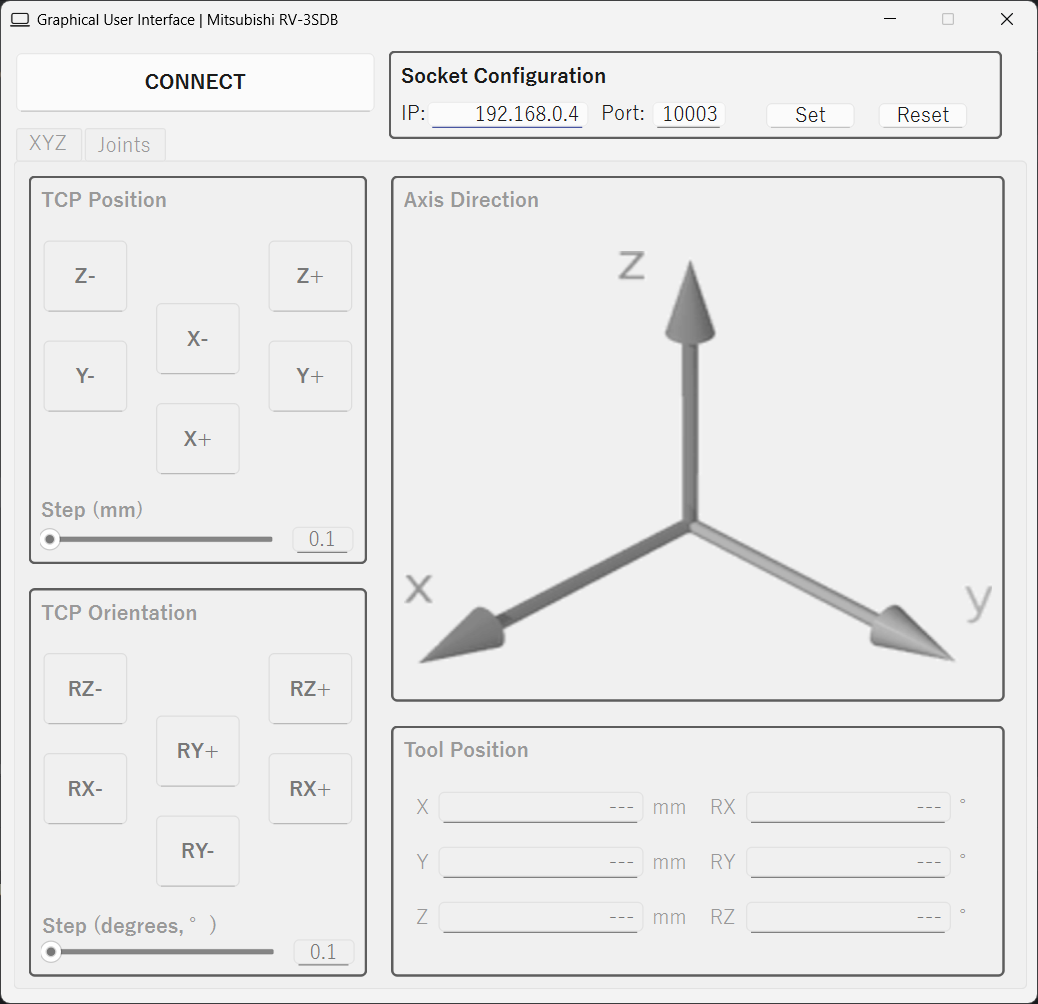
\includegraphics[scale=0.5]{nonactive.png}
    \caption{Окно клиентской программы до подключения к роботу.}
    \label{fig:nonactive}
\end{figure}
\begin{figure}[H]
    \centering
    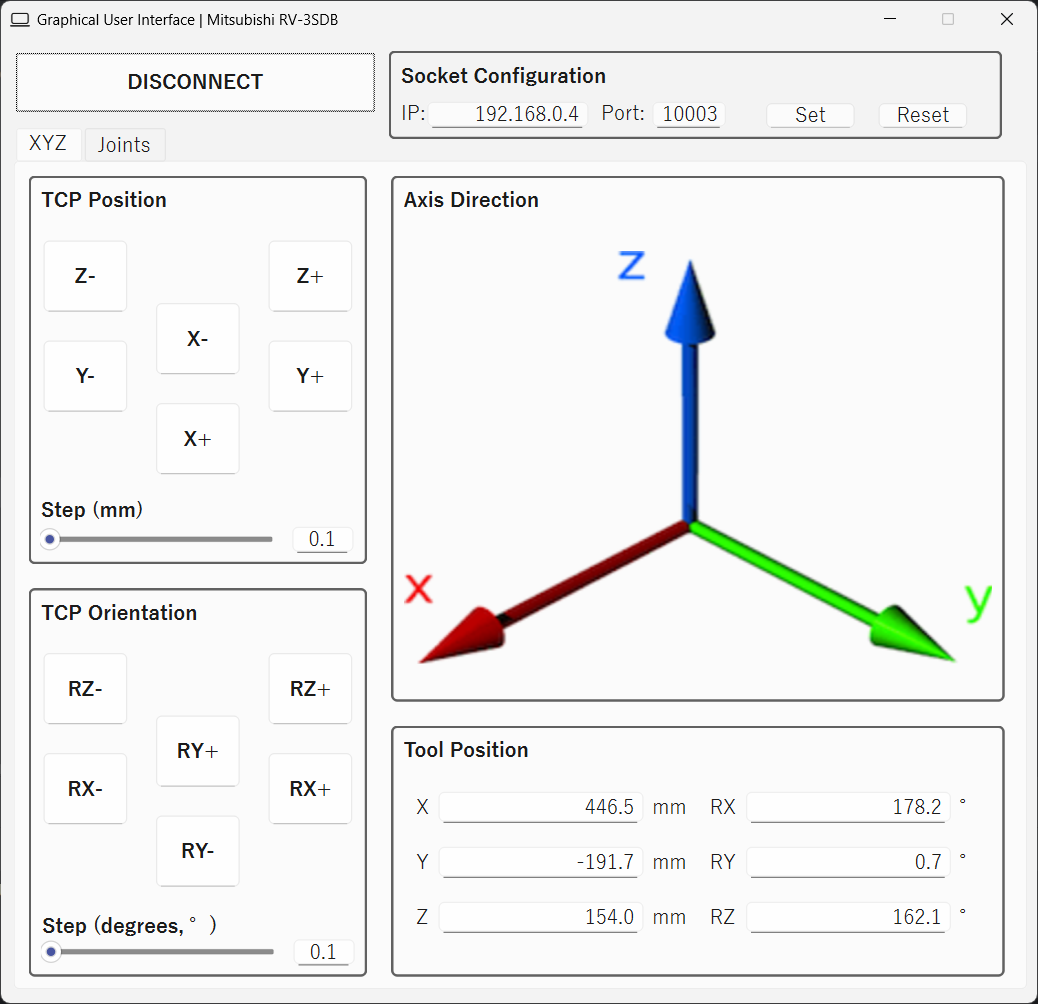
\includegraphics[scale=0.5]{active_cartesian.png}
    \caption{Окно клиентской программы после подключения к роботу: декартовы координаты.}
    \label{fig:active_cartesian}
\end{figure}


Для сочлененных координат необходимо поменять вкладку 'XYZ' на 'Joints'.
Окно программы с переключением на сочлененные координаты имеет вид:
\begin{figure}[H]
    \centering
    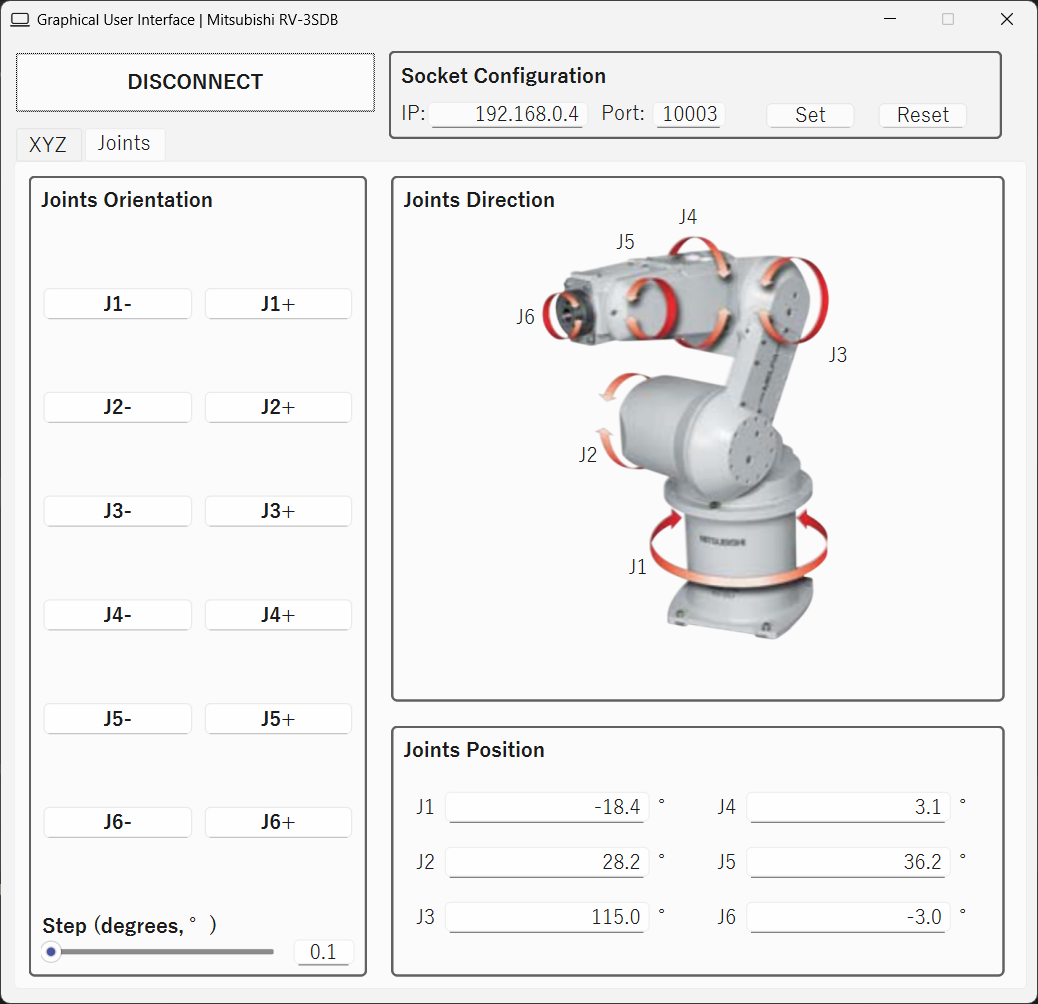
\includegraphics[scale=0.5]{active_joint.png}
    \caption{Окно клиентской программы после подключения к роботу: сочлененные координаты.}
    \label{fig:active_joint}
\end{figure}


Проверим соответствие координат в программе координатам, отображаемым на пульте управления.
\begin{figure}[H]
    \centering
    \includegraphics[scale=0.06]{cartesian_pult.png}
    \caption{Проверка соответствия координат: декартовы координаты на пульте.}
    \label{fig:cartesian_pult}
\end{figure}
\begin{figure}[H]
    \centering
    \includegraphics[scale=0.06]{joint_pult.png}
    \caption{Проверка соответствия координат: сочлененные координаты на пульте.}
    \label{fig:joint_pult}
\end{figure}


Сравнивая рис. \ref{fig:cartesian_pult} с \ref{fig:active_cartesian}
и \ref{fig:joint_pult} с \ref{fig:active_joint} видим, что координаты
совпадают с учетом округления.


Зафиксируем начальное положение робота.
Несколько раз нажмем кнопку 'Y+' в окне программы, задав ползунком шаг 5 мм.
Зафиксируем конечное положение робота.
\begin{figure}[H]
    \centering
    \includegraphics[scale=0.06]{cartesian_Y_1.png}
    \caption{Начальное положение робота.}
    \label{fig:cartesian_Y_1}
\end{figure}
\begin{figure}[H]
    \centering
    \includegraphics[scale=0.06]{cartesian_Y_2.png}
    \caption{Положение робота после нажатия кнопки 'Y+' несколько раз с шагом 5 мм.}
    \label{fig:cartesian_Y_2}
\end{figure}


Как видим, робот переместился вдоль координаты 'Y'. При автоматическом
управлении роботом ручной режим недоступен.


\subsection{Проблемы в ходе тестирования}
В ходе тестирования работоспособности программы
случались некоторые ошибки, в основном связанные
с проверкой условий, обработкой ответа от робота
или несовпадением ожидаемых и получаемых типов переменных
внутри клиентской логики.
Все проблемы были решены на месте, программа стала работать без ошибок.


\section{Заключение}
В ходе выполнения практической работы
были разработаны алгоритмы для взаимодействия
компьютера с роботом-манипулятором,
их работоспособность была успешно проверена на роботе.
Для выполнения работы был изучен робот-манипулятор,
язык программирования MELFA BASIC
и сетевое взаимодействие с помощью
языка программирования Python.
Был выбран формат сообщения,
простестирована связь клиента и робота,
доработана основная логика, подключен
графический интерфейс и отлажены ошибки,
возникшие в процессе тестирования.


\section{Список использованных источников}
\begin{enumerate}
    \item Mitsubishi Electric MELFA RV-3SDB Series Manuals \href{https://www.manualslib.com/products/Mitsubishi-Electric-Melfa-Rv-3sdb-Series-11307307.html}{(ссылка)}
    \item socket -- Low-level networking interface \href{https://docs.python.org/3/library/socket.html}{(ссылка)}
    \item re — Regular expression operations \href{https://docs.python.org/3/library/re.html}{(ссылка)}
    \item typing — Support for type hints \href{https://docs.python.org/3/library/typing.html}{(ссылка)}
    \item enum — Support for enumerations \href{https://docs.python.org/3/library/enum.html}{(ссылка)}
    \item Python YAML: How to Load, Read, and Write YAML \href{https://python.land/data-processing/python-yaml}{(ссылка)}
\end{enumerate}


\appendix
\renewcommand{\thesection}{\Asbuk{section}}

\section{Приложение}
\begin{lstlisting}[label=lst:client, caption={Основа для общения компьютера с роботом.}]
import socket
import connection_status as cs

class Client:
    def __init__(self):
        self.sock = socket.socket(socket.AF_INET, socket.SOCK_STREAM)
        self.connected = False

    def connect(self, ip: str, port: int) -> cs.ConnectionStatus:
        try:
            self.sock.connect((ip, port))
            self.connected = True

            return cs.ConnectionStatus.SUCCESS
        except socket.error:
            self.connected = False

            return cs.ConnectionStatus.CONNECTION_ERROR

    def disconnect(self) -> cs.ConnectionStatus:
        if self.connected:
            try:
                self.sock.close()
                self.connected = False

                return cs.ConnectionStatus.SUCCESS
            except socket.error:
                return cs.ConnectionStatus.CONNECTION_ERROR
        
        return cs.ConnectionStatus.NOT_CONNECTED

    def send(self, data: str) -> cs.ConnectionStatus:
        if not self.connected:
            return cs.ConnectionStatus.NOT_CONNECTED
        try:
            self.sock.sendall(data.encode('utf-8'))

            return cs.ConnectionStatus.SUCCESS
        except socket.error:
             return cs.ConnectionStatus.SEND_ERROR

    def receive(self, out_data: list, buffer_size: int = 1024) -> cs.ConnectionStatus:
        if not self.connected:
            return cs.ConnectionStatus.NOT_CONNECTED
        try:
            received = self.sock.recv(buffer_size)
            out_data.clear()
            out_data.append(received.decode('utf-8'))

            return cs.ConnectionStatus.SUCCESS
        except socket.error:
            return cs.ConnectionStatus.RECEIVE_ERROR
\end{lstlisting}


\section{Приложение}
\begin{lstlisting}[label=lst:cmdman, caption={Скрипт с функциями для обработки координат на отправку или получение.}]
from typing import List
import re

class CommandMessageManager:
    @staticmethod
    def build_position_request(pos: List[float]) -> str:
        if len(pos) != 6:
            raise ValueError('List of pos must contain 6 values')

        return f"({','.join(map(str, pos))})"

    @staticmethod
    def parse_position_response(response: list):
        try:
            matches = re.findall(r'\((.*?)\)', response[0])
            lists = [list(map(float, group.split(','))) for group in matches[:2]]
            lists.append(list(map(int, matches[2].split(','))))

            return tuple(lists)
        except ValueError:
            return None
\end{lstlisting}


\section{Приложение}
\begin{lstlisting}[label=lst:cfg, caption={Скрипт для работы с чтением и сохранением конфигурации IP и порта робота.}]
import yaml

class Config:
    ip: str = ""
    port: int = 0

    @classmethod
    def load(cls, path: str = "config.yaml"):
        with open(path, "r") as file:
            config = yaml.safe_load(file)
            cls.ip = config["connection"]["ip"]
            cls.port = config["connection"]["port"]

    @classmethod
    def save(cls, path: str = "config.yaml"):
        with open(path, "w") as file:
            yaml.safe_dump({
                "connection": {
                    "ip": cls.ip,
                    "port": cls.port
                }
            }, file)

    @classmethod
    def set_config(cls, ip: str, port: int):
        cls.ip = ip
        cls.port = port
\end{lstlisting}


\section{Приложение}
\begin{lstlisting}[label=lst:virtualrobot, caption={Скрипт виртуального робота: сохранение координат робота и кинематической пары. Вычисление следующих координат по индексу и шагу.}]
from typing import List, Literal, Tuple

class VirtualRobot:
    def __init__(self,
                 cartesian: List[float] = None,
                 joint: List[float] = None,
                 kin_sol: Tuple[int, int] = None):
        self.cartesian = cartesian if cartesian is not None else [0.0] * 6
        self.joint = joint if joint is not None else [0.0] * 6
        self.kinematic_sol = kin_sol if kin_sol is not None else (0, 0)

    def update_cartesian(self, new_values: List[float], kinematic_sol: Tuple[int, int]):
        if len(new_values) != 6:
            raise ValueError("Cartesian must have 6 values")
        self.cartesian = new_values.copy()
        self.kinematic_sol = kinematic_sol

    def update_joint(self, new_values: List[float]):
        if len(new_values) != 6:
            raise ValueError("Joint must have 6 values")
        self.joint = new_values.copy()

    def calculate_next_move(
        self,
        mode: Literal["cartesian_linear", "cartesian_rotation", "joint_rotation"],
        axis_index: int,
        step: float
    ) -> List[float]:
        if not (0 <= axis_index < 6):
            raise ValueError("Value of axis_index must be in range from 0 to 5")

        if "cartesian" in mode:
            new_pos = self.cartesian.copy()
        elif "joint" in mode:
            new_pos = self.joint.copy()
        else:
            raise ValueError("Expected 'cartesian' or 'joint' mode")

        new_pos[axis_index] += step
        return new_pos
\end{lstlisting}


\section{Приложение}
\begin{lstlisting}[label=lst:backctrl, caption={Скрипт, объединяющий различные функции для полноценного взаимодействия с роботом с компьютера.}]
from typing import Tuple, Literal

from virtual_robot import VirtualRobot
from command_manager import CommandMessageManager
from robot_command import RobotCommand, MODE_TO_COMMAND
from client import Client
from connection_status import ConnectionStatus

class BackendController:
    def __init__(self):
        self.robot = VirtualRobot()
        self.client = Client()
        self.last_connection_status = ConnectionStatus.NONE
        self.last_cmd_send_status = ConnectionStatus.NONE
        self.last_params_send_status = ConnectionStatus.NONE
        self.last_receive_status = ConnectionStatus.NONE

    def connect(self, ip: str, port: int):
        self.last_connection_status = self.client.connect(ip, port)
        return self.client.connected

    def disconnect(self):
        cmd = str(RobotCommand.EXIT.value)
        self.last_cmd_send_status = self.client.send(cmd)
        
        self.last_connection_status = self.client.disconnect()
        
        return not self.client.connected

    def is_connected(self):
        return self.client.connected

    def get_pos(self):
        cmd = str(RobotCommand.GET_POSITION.value)
        self.last_cmd_send_status = self.client.send(cmd)

        ans = []
        self.last_receive_status = self.client.receive(ans)

        return ans

    def move_axis(self,
                  move_info: Tuple[Literal["cartesian_linear", "cartesian_rotation", "joint_rotation"], int, Literal['+', '-']],
                  step: float):
        mode, axis_index, direction = move_info

        signed_step = step if direction == '+' else -step
        pos = self.robot.calculate_next_move(mode, axis_index, signed_step)

        cmd = str(MODE_TO_COMMAND[mode].value)

        params = CommandMessageManager.build_position_request(pos)
        if "cartesian" in mode:
            params = f"{params}({','.join(map(str, self.robot.kinematic_sol))})"

        self.last_cmd_send_status = self.client.send(cmd)
        self.last_params_send_status = self.client.send(params)

        ans = []
        self.last_receive_status = self.client.receive(ans)

        return ans
\end{lstlisting}


\section{Приложение}
\begin{lstlisting}[language=Basic, label=lst:finalmelfa, caption={Программа на роботе-манипуляторе для выполнения команд, присылаемых клиентом.}]
JOVRD 100
SPD 100
DEF INTE DCOMM
DCOMM = 1
PHELP = P_CURR
JHELP = J_CURR
SERVO ON
OPEN "COM3:" AS #1

WHILE DCOMM > 0
    INPUT #1, DCOMM
    IF DCOMM = 1 THEN
        PRINT #1, J_CURR, P_CURR
    ENDIF
    IF DCOMM = 2 THEN
        INPUT #1, PHELP
        MOV PHELP
        PRINT #1, J_CURR, P_CURR
    ENDIF
    IF DCOMM = 3 THEN
        INPUT #1, JHELP
        MOV JHELP
        PRINT #1, J_CURR, P_CURR
    ENDIF
WEND

CLOSE #1
SERVO OFF
END
\end{lstlisting}


\section{Приложение}
\begin{lstlisting}[label=mvinf, caption={Карта кнопок окна программы, которым соответствуют кортежи move\_info, описывающие соответствующую кнопку.}]
self.axis_button_map = {
'btn_Xp': ("cartesian_linear", CartesianAxis.X.value, '+'),
'btn_Xm': ("cartesian_linear", CartesianAxis.X.value, '-'),
'btn_Yp': ("cartesian_linear", CartesianAxis.Y.value, '+'),
'btn_Ym': ("cartesian_linear", CartesianAxis.Y.value, '-'),
'btn_Zp': ("cartesian_linear", CartesianAxis.Z.value, '+'),
'btn_Zm': ("cartesian_linear", CartesianAxis.Z.value, '-'),
'btn_RXp': ("cartesian_rotation", CartesianAxis.A.value, '+'),
'btn_RXm': ("cartesian_rotation", CartesianAxis.A.value, '-'),
'btn_RYp': ("cartesian_rotation", CartesianAxis.B.value, '+'),
'btn_RYm': ("cartesian_rotation", CartesianAxis.B.value, '-'),
'btn_RZp': ("cartesian_rotation", CartesianAxis.C.value, '+'),
'btn_RZm': ("cartesian_rotation", CartesianAxis.C.value, '-'),
'btn_J1p': ("joint_rotation", JointAxis.J1.value, '+'),
'btn_J1m': ("joint_rotation", JointAxis.J1.value, '-'),
'btn_J2p': ("joint_rotation", JointAxis.J2.value, '+'),
'btn_J2m': ("joint_rotation", JointAxis.J2.value, '-'),
'btn_J3p': ("joint_rotation", JointAxis.J3.value, '+'),
'btn_J3m': ("joint_rotation", JointAxis.J3.value, '-'),
'btn_J4p': ("joint_rotation", JointAxis.J4.value, '+'),
'btn_J4m': ("joint_rotation", JointAxis.J4.value, '-'),
'btn_J5p': ("joint_rotation", JointAxis.J5.value, '+'),
'btn_J5m': ("joint_rotation", JointAxis.J5.value, '-'),
'btn_J6p': ("joint_rotation", JointAxis.J6.value, '+'),
'btn_J6m': ("joint_rotation", JointAxis.J6.value, '-'),
} 
\end{lstlisting}


\section{Приложение}
\begin{lstlisting}[label=lst:hancon, caption={Реализация обработки нажатия на кнопку connect/disconnect в интерфейсе.}]
def handle_connection(self):
    if self.backend.is_connected():
        self.backend.disconnect()

        if not self.backend.is_connected():
            self.ui.tabWidget.setEnabled(False)
            self.ui.btn_connect.setText("CONNECT")
    else:
        try:
            ip = Config.ip
            port = Config.port
            self.backend.connect(ip, port)

            if self.backend.is_connected():
                response = self.backend.get_pos()
                joints, cartesian, kinematic_sol = CommandMessageManager.parse_position_response(response)

                self.backend.robot.update_cartesian(cartesian, kinematic_sol)
                self.backend.robot.update_joint(joints)

                self.update_ui_axis()

                self.ui.tabWidget.setEnabled(True)
                self.ui.btn_connect.setText("DISCONNECT")
        except Exception as e:
            print(f"Caught exception: {e}")
\end{lstlisting}


\section{Приложение}
\begin{lstlisting}[label=lst:hab, caption={Реализация функции обработки нажатия кнопок изменения координат.}]
def handle_axis_button(self):
    btn = self.sender()
    if not btn:
        return

    btn_name = btn.objectName()
    if btn_name not in self.axis_button_map:
        print(f"Unexpected button: {btn_name}")
        return

    move_info = self.axis_button_map[btn_name]
    mode, _, _ = move_info

    if "cartesian" in mode:
        if not "rotation" in mode:
            step = self.linear_step_val
        else:
            step = self.degree_1_step_val
    else:
        step = self.degree_2_step_val

    if not self.backend.is_connected():
        print("Unexpected event: no connection")
        return

    try:
        response = self.backend.move_axis(move_info, step)
        joints, cartesian, kinematic_sol = CommandMessageManager.parse_position_response(response)

        self.backend.robot.update_cartesian(cartesian, kinematic_sol)
        self.backend.robot.update_joint(joints)

        self.update_ui_axis()
    except Exception as e:
        print(f"Caught exception: {e}")
\end{lstlisting}
\end{document}